\documentclass[wi]{zut}

\usepackage{microtype}
\usepackage{wrapfig}

\author{Karol Działowski}
\title{Pytania na obronę pracy magisterskiej}

\makemetadata

\begin{document}

\maketitle
\tableofcontents

\section{Wstęp}

Poniższe opracowania były opracowywane indywidualnie i nie są oficjalnymi ani sprawdzonymi odpowiedziami na pytania. Na wiele pytań nie jestem pewien udzielonej odpowiedzi -- przy nich widnieje znak zapytania jak na przykładzie niżej.

W tym akapicie przedstawiony jest schemat oznaczenia pytań co do których odpowiedzi nie mam pewności. Po prawej stronie będzie wklejona ikona znaku zapytania.
\question

Podczas opracowywania pytań starałem się tłumaczyć możliwie jak najogólniej powiązane zagadnienia. W wielu przypadkach też zamieściłem odnośniki do źródeł z których korzystałem podczas tworzenia z tego dokumentu.

% \section{Przedmioty wspólne}

% \subsection{Zasady cyfryzacji sygnałów. Prawo Kotielnikowa-Shannona. Granica Nyquisa. Aliasing.}
% Aleksandr Cariow. Cyfrowe przetwarzanie sygnałów.

% \subsection{Bezpieczny schemat podpisu cyfrowego. Modele bezpieczeństwa.}
% Tomasz Hyla. Kryptologia.

% \subsection{Idea interpolacji funkcji z wykorzystaniem funkcji sklejanych.}
% Piotr Piela. Matematyka obliczeniowa.

% \subsection{Styl poznawczy (kognitywny) człowieka}
% Izabela Rejer. Wprowadzenie do kognitywistyki.

% \subsection{Korzyści wynikające z zastosowania grafowych baz danych do przetwarzania dużych zbiorów danych o strukturach grafowych}
% Przemysław Korytkowski. Duże zbiory danych.

% \subsection{Założenia i obszary zastosowania platformy Apache Spark}
% Przemysław Korytkowski. Duże zbiory danych.

% \subsection{Sposoby sprawdzenia właściwości losowych danego ciągu}
% Tomasz Hyla. Kryptologia.

% \subsection{Filtracja cyfrowa: filtry SOI i NOI}
% Aleksandr Cariow. Cyfrowe przetwarzanie sygnałów.

% \subsection{Reprezentacja sygnałów za pomocą szeregów funkcyjnych. Dyskretne transformacje ortogonalne oraz szybkie algorytmy ich wyznaczania.}
% Aleksandr Cariow. Cyfrowe przetwarzanie sygnałów.

% \subsection{Atak na podpis cyfrowy wykorzystujący paradoks dnia urodzin}
% Tomasz Hyla. Kryptologia.

% \subsection{Podział metod rozwiązywania równań liniowych metodami numerycznymi}
% Piotr Piela. Matematyka obliczeniowa.

% \subsection{Algorytm numeryczny niestabilny a algorytm źle uwarunkowany}
% Piotr Piela. Matematyka obliczeniowa.

% \subsection{Programowanie kodu wielowątkowego wraz z wzajemnym wykluczaniem w C++ 11 Threads}
% Marek Pałkowski. Obliczenia dużej mocy.

% \subsection{Cechy środowiska Hadoop}
% Przemysław Korytkowski. Duże zbiory danych.

% \subsection{Rodzaje błędów składające się na całkowity błąd obliczeń numerycznych}
% Piotr Piela. Matematyka obliczeniowa.

% \subsection{Standard C++ 17 Parallel}
% Marek Palkowski. Obliczenia dużej mocy.

% \subsection{Dokładność rozwiązywania równań różniczkowych metodami numerycznymi}
% Piotr Piela. Matematyka obliczeniowa.

% \subsection{Wpływ zachowań z obszaru kognitywistyki relacji społecznych na rozwój mediów społecznościowych}
% Izabela Rejer. Wprowadzenie do kognitywistyki.

% \subsection{Programowanie przenośnego kodu wielowątkowego na przykładzie PosixThreads}
% Marek Pałkowski. Obliczenia dużej mocy.

% \subsection{Zastosowanie okulografii w pięciu wybranych dziedzinach życia}
% Izabela Rejer. Wprowadzenie do kognitywistyki.

\section{Inteligencja obliczeniowa}

% \subsection{Charakterystyka języków programowania wykorzystywanych w analizie danych}
% Marcin Pluciński. Języki analizy danych.

% \subsection{Porównanie dwóch dowolnych algorytmów wykrywania obiektów}
% Paweł Forczmański. Widzenie komputerowe.

% \subsection{Charakterystyka wybranych metod śledzenia obiektów}
% Paweł Forczmański. Widzenie komputerowe.

\subsection{Trzy pytania, na które odpowiadają Ukryte Modele Markowa oraz używane do tego celu algorytmy}
% Marcin Pietrzykowski. Eksploracja danych.

Na początku warto przypomnieć co to Ukryte Modele Markowa. Model Markowa składa się z $N$ stanów $S$, które są ukryte oraz $M$ obserwacji $V$. Podobnie jak w łańcuchu Markowa w każdym momencie czasowym model może być w jednym stanie. Prawdopodobieństwa przejścia pomiędzy stanami zależą tylko od stanu poprzedniego. Dla każdego stanu system generuje obserwacje z danym prawdopodobieństwem \cite{Pietrzykowski2020}. 

Modele Markowa są dobre do rozpoznawania zmiennych wzorców, np. mowa, pismo odręczne, gesty, predykcja genów itd.\cite{Pietrzykowski2020}

\begin{figure}[H]
    \centering
    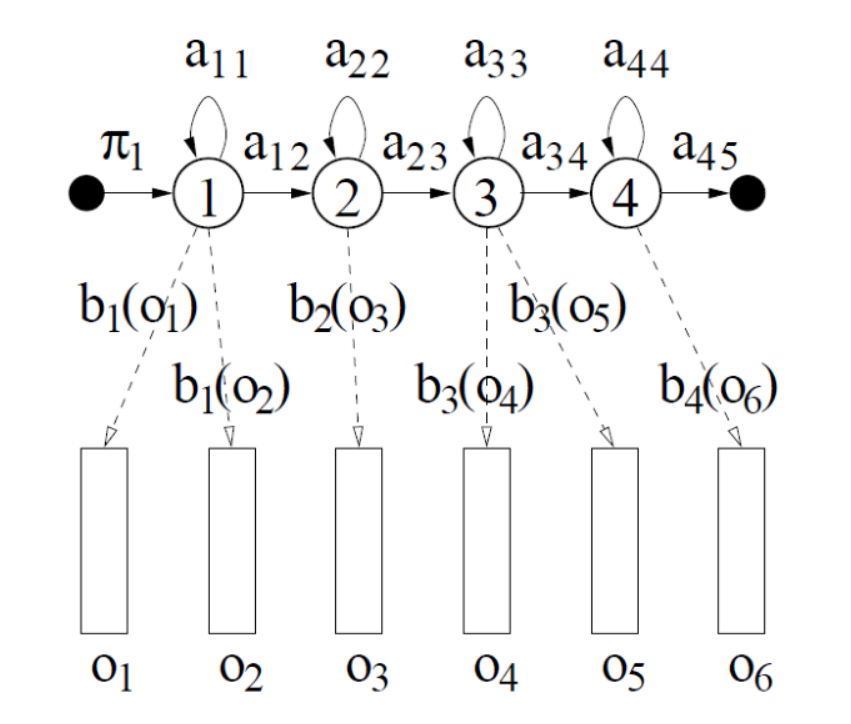
\includegraphics[width=0.5\linewidth]{images/hidden_markov.png}
    %\vspace{1em}
    \caption{Przykładowe reprezentacja Ukrytego Modelu Markowa. Prostokąty to obserwacje, kółka to stany ukryte.}
    \label{fig:pdgd}
    \source{M. Pietrzykowski. Wykład 4 - Ukryte Modele Markowa. \cite{Pietrzykowski2020}}
\end{figure}

\subsubsection{Mając sekwencję obserwacji $O = (O_1, O_2, \ldots, O_T)$ i model $\lambda = (A, B, \pi)$ jakie jest prawdopodobieństwo tej sekwencji pod warunkiem tego modelu, czyli $P(O|\lambda)$}

Prawdopodobieństwo $P(O|\lambda)$ musi być wyznaczone używając formuła na całkowite prawdopodobieństwo, tj. brać pod uwagę wszystkie możliwe ścieżki stanów. Takie przeszukiwanie w sposób zachłanny jest niemożliwe w praktyce. Złożoność obliczeniowa wynosi $O(TN^T)$\cite{Pietrzykowski2020}. 

W praktyce to zadanie rozwiązuje się za pomocą algorytmu \textbf{Forward-Backward}. Jego złożoność jest rzędu $O(TN^2)$\cite{Pietrzykowski2020}.

\subsubsection{Mając sekwencję obserwacji $O = (O_1, O_2, \ldots, O_T)$ i model $\lambda = (A, B, \pi)$ jak dobieramy najlepszą sekwencję stanów $Q = (q_1, q_2, \ldots, q_T)$, która odpowiada sekwencji obserwacji O?}

Mając sekwencję obserwacji należy odpowiedzieć jaka jest najbardziej prawdopodobna sekwencja stanów ukrytych uwzględniając model (tj. prawdopodobieństwa przejść oraz prawdopodobieństwa obserwacji).

Aby odpowiedzieć na to pytanie używamy algorytmu \textbf{Viterbiego} bazujący na metodach programowania dynamicznego. Jego celem jest znalezienie jednego najlepszej sekwencji stanów, która maksymalizuje $P(Q, O|\lambda)$~\cite{Pietrzykowski2020}.

\subsection{Mając sekwencję obserwacji $O = (O_1, O_2, \ldots, O_T)$ i znając tylko $M$ i $N$ (liczba obserwacji i stanów) jak stroić model?}

Jak dobrać najlepsze zmienne modelu $\lambda = (A, B, \pi)$ aby zmaksymalizować $P(O|\lambda)$?

Mamy sekwencję obserwacji, wiedząc ile ma być stanów i obserwacji jak nastroić model?

Jest to najtrudniejszy z problemów. W tym celu używa się podejścia iteracyjnego nazwanego \textbf{metodą Bauma-Welcha}~\cite{Pietrzykowski2020}.

% \subsection{Cechy obiektów audio i metody ekstrakcji cech tych obiektów}
% Edward Półroliczak. Ekstrakcja cech.

% \subsection{Przebieg uczenia ze wzmocnieniem i pozyskiwana w tym procesie wiedza}
% Marcin Pluciński. Uczenie maszynowe 2.

\subsection{Cechy charakterystyczne splotowych sieci neuronowych}
% Paweł Forczmański. Uczenie maszynowe 2.

\textbf{Convolution Neural Networks} (CNN, ConvNet) to wariant MLP inspirowany biologicznie, gdzie mnożenie wag i sygnału wejściowe zastąpione jest operacją \textbf{splotu} \cite{Forczmanski2020}.

Cechami charakterystycznymi splotowych sieci są:

\begin{itemize}
    \item rzadka reprezentacja
    \item współdzielone wagi
    \item pooling (zmniejszanie rozdzielczości, np. wybierając maksymalną wartość z danego sąsiedztwa)
\end{itemize}

Sieci te potrafią stopniowo filtrować różne części danych i wyostrzać ważne fragmenty w procesie dyskryminacji (rozpoznawanie/klasyfikacja wzorców) \cite{Forczmanski2020}.

Sieci splotowe są łatwiejsze do uczenia, gdyż zawierają mniej parametrów (wykorzystują te same wagi) niż typowe sieci neuronowe \cite{Forczmanski2020}. 

Wykorzystywanie głównie do obliczeń na strukturach dwuwymiarowych (np. obrazy) \cite{Forczmanski2020}.

\begin{figure}[H]
    \centering
    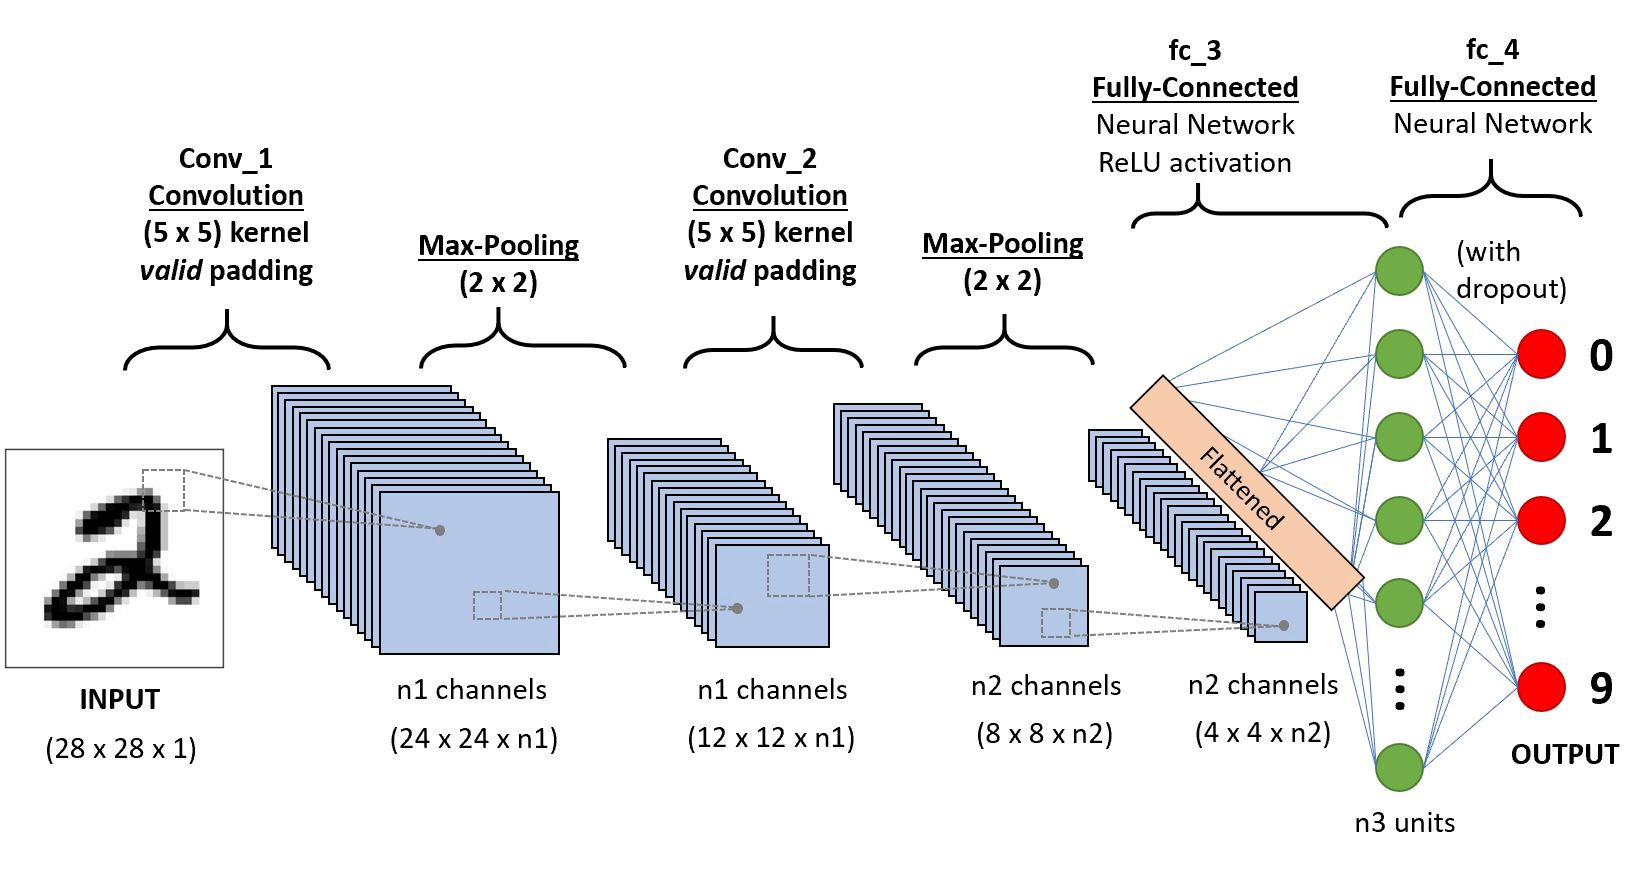
\includegraphics[width=0.7\linewidth]{images/cnn.jpeg}
    %\vspace{1em}
    \caption{Przykładowe architektura sieci splotowej.}
    \label{fig:cnn}
    \source{\url{https://datasciencepr.com/convolutional-neural-network/}}
\end{figure}

Pojedynczy neuron (jednostka obliczeniowa) w sieciach splotowych definiuje się za pomocą:

\begin{itemize}
    \item szerokości,
    \item wysokości,
    \item głębokości (liczba filtrów),
    \item stride (krok przesunięcia filtru) \cite{Forczmanski2020}.
\end{itemize}

% \subsection{Podstawowe różnice między sygnałem mowy a sygnałem muzycznym w dziedzinie częstotliwości}
% Tomasz Mąka. Sygnały akustyczne.

\subsection{Metody próbkowania sieci złożonych}
% Jarosław Jankowski. Sieci złożone.

To jest dziwne, bo to pytanie z przedmiotu \emph{Duże zbiory danych}, które były przedmiotem wspólnym.

Próbkowanie i agregacja dają możliwość rozwiązaniem problemu bardzo dużych zbiorów grafowych. Przykładowo chcąc analizować sieć połączeń na Facebooku, reprezentowaną przez ponad 1 miliard węzłów, potrzebowalibyśmy 1TB pamięci aby zapisać same relacje w postaci grafu, bez atrybutów, etykiet i treści~\cite{Jankowski2020_probkowanie}. 

W próbkowaniu sieci informacja o węzłach jest pozyskiwana dopiero po pobraniu danej próbki, \textbf{struktura całej sieci nie jest znana}. Wymagana jest strategia eksploracji sieci i stopniowego powiększania próbki. Celem próbkowania jest stopniowa identyfikacja małego zbioru przedstawicieli węzłów i powiązań ze struktury sieciowej, przy posiadanej niewielkiej wiedzy o całej sieci. W skrócie jest to uogólnienie sieci, stworzenie modelu sieci, która zachowuje \textbf{niektóre właściwości} sieci pierwotnej~\cite{Jankowski2020_probkowanie}. 

Przy agregacji cała struktura sieci musi być znana apriori. Celem agregacji są miary, które umożliwiają opis własności sieci na poziomie ogólnym~\cite{Jankowski2020_probkowanie}. 

W próbkowaniu sieci homogenicznych (jednorodnych) wyróżniamy dwie główne strategie:

\begin{itemize}
    \item Wybór węzłów lub krawędzi o zadanych właściwościach
    \begin{itemize}
        \item Losowy wybór węzłów
        \item Na podstawie stopnia wierzchołka (prawdopodobieństwo proporcjonalne do stopnia)
        \item Na podstawie miary PageRank
    \end{itemize}
    \item Pobieranie próbek w procesie eksploracji
    \begin{itemize}
        \item Random Walk - rekurencyjnie wybierany losowo tylko jeden z sąsiadów
        \item Snowball sampling - rekurencyjnie włączamy $n$ sąsiadów
        \item Poszukiwanie wzorców
    \end{itemize}
\end{itemize}

W sieciach heterogenicznych (niejednorodnych) możemy skorzystać z \emph{multi-graph sampling}, pobierania próbek z zachowaniem rozkładu typów, próbkowania z zachowaniem relacji~\cite{Jankowski2020_probkowanie}.


% \subsection{Elementy składowe procesu klasyfikacji sygnałów akustycznych}
% Tomasz Mąka. Sygnały akustyczne.

% \subsection{Model SVM (procedura uczenia, wariant liniowy i nieliniowy, przekształcenia jądrowe).}
% Marcin Korzeń. Uczenie maszynowe 1.

% \subsection{Sieci perceptronowe i metody uczenia perceptronu (warianty algorytmów uczenia, głosowanie, zastosowania)}
% Marcin Korzeń. Uczenie maszynowe 1.

% \subsection{Proces tworzenia zbioru uczącego, walidującego i testowego w głębokim uczeniu}
% Paweł Forczmański. Uczenie maszynowe 2.

% \subsection{Sposób działania algorytmów uczących AdaBoost i RealBoost}
% Przemysław Klęsk. Uczenie maszynowe 2.

% \subsection{Omówienie na przykładzie algorytmu Apriori odkrywania asocjacji w zbiorach danych}
% Joanna Kołodziejczyk. Eksploracja danych.

% \subsection{Przykład siedzi bayesowskiej (przekonań): struktura sieci, właściwości i jej interpretacja oraz uczenie}
% Joanna Kołodziejczyk. Eksploracja danych.

\subsection{Deskryptory cech niskopoziomowych - wybrane algorytmy w odniesieniu do wykorzystywanych cech}
% Dariusz Frejlichowski. Ekstrakcja cech.

Deskryptory cech odnoszą się do zagadnienia ekstrakcji cech. Deskryptor opisuje daną cechę za pomocą wartości numerycznych. Poniżej opisywano tylko deskryptory odnoszące się do obrazów. Oprócz tego istnieją inne deskryptory, np. w rozpoznawaniu dźwięku częstotliwość fundamentalna, formanty, itd.

\textbf{Atrybuty niższego poziomu abstrakcji} - metadane typu sygnałowego, są wartościowane przez komputer (np. kolor dominujący, histogram krawędzi, aktywność ruchu w obrazie, czy linia melodyczna utworu muzycznego) \cite{Frejlichowski2020}.

Standard MPEG-7 opisuje między innymi deskryptory wizualne. Deskryptory wizualne MPEG-7 opisują na \textbf{niewielu} bitach obrazy, sekwencje obrazów, obszary w obrazie itd. 

Deskryptor powinien być:

\begin{itemize}
    \item efektywny i ekspresyjny (porównywalny z widzeniem u ludzi),
    \item zwarty (w aspekcie pamięci),
    \item o małej złożoności ekstrakcji i zapytań \cite{Frejlichowski2020}.
\end{itemize}

Wyróżniamy następujący podział deskryptorów:

\begin{itemize}
    \item \textbf{Koloru} - Scalable Color, Color Structure, Dominant Color, histogramy,
    \item \textbf{Kształtu} - sygnatura, UNL, UNL-F, mUNL,
    \item \textbf{Odcieni szarości} - Polar-Fourier Greyscale Descriptor, Rzutowanie wartości,
    \item \textbf{Ruchu},
    \item \textbf{Tekstury}.
\end{itemize}

\subsubsection{Deskryptory kształtu}

Główne problemy z deskryptorami kształtu to:

\begin{itemize}
    \item obrót, skalowanie, przesunięcie (przekształcenia afiniczne)
    \item szum,
    \item nieciągłości,
    \item okluzja.
\end{itemize}

Czyli najlepszy deskryptor jest inwariantny względem obrotu, skalowania, przesunięcia oraz jest niewrażliwy na szum i okluzję.

Proste deskryptory kształtu to m.in. pole powierzchni, długość obwodu, kołowość, zwartość, mimośród, powłoka wypukła, object aspect ratio, itd. \cite{Frejlichowski2020_2}

Przykładowym deskryptorem jest UNL-F. Zapewnia on dobrą odporność na szum, przekształcenia afiniczne (transformata Fouriera daje odporność na obrót). Jedyną wadą jest brak odporności na okluzję. W pewnym stopniu rozwiązuje to mUNL, który zmienia podejście do wyznaczania centroidu  \cite{Frejlichowski2020_2}.

W skrócie UNL-F składa się on z następujących kroków:

\begin{enumerate}
    \item Binaryzacja obiektu
    \item Wyznaczenie centroidu
    \item Przekształcenie do współrzędnych polarnych
    \item Wycinek widma po transformacie 2D Fouriera -- tego kroku nie ma w zwykłej metodzie UNL
\end{enumerate}

\begin{figure}[H]
    \centering
    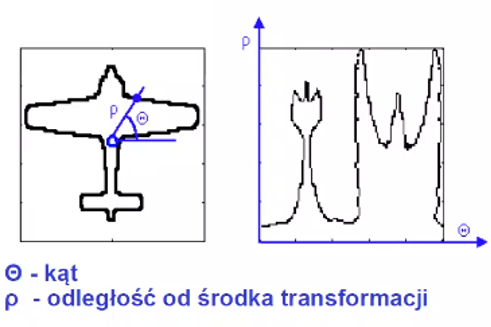
\includegraphics[width=0.5\linewidth]{images/unl.png}
    \caption{Działanie deskryptora UNL}
    \label{fig:unl}
    \source{Wykład 2 - D. Frejlichowski \cite{Frejlichowski2020_2}}
\end{figure}

\subsubsection{Deskryptory koloru}

Przykładowe deskryptory koloru ze standardu MPEG-7 to:

\begin{itemize}
    \item Deskryptor koloru dominującego
    \item Skalowalny deskryptor koloru
    \item Deskryptor GOF i GOP
    \item Deskryptor struktury koloru
    \item Deskryptor widoku koloru (layout)
    \item Temperatura barwowa \cite{Frejlichowski2020_6}
\end{itemize}

Inne deskryptory koloru to:

\begin{itemize}
\item histogram RGB lub HSV - może dawać takie same wyniki dla różnych obrazów
\item IBOX8
\item DHV
\item RGBBOX8
\item RGBI \cite{Frejlichowski2020_6}
\end{itemize}

Przykładowo, deskryptor koloru dominującego polega na wyznaczenie $n$ kolorów dominujących dla obrazu za pomocą algorytmu $k$-means i obliczenie ich udziałów \cite{Frejlichowski2020_6}.

Skalowalny deskryptor koloru bazuje na przestrzeni barw HSV i transformacji Haara zastosowanej na wartościach histogramu koloru \cite{Frejlichowski2020_6}.

Deskryptor rozkładu koloru (Color Layout Descriptor) uchwyca rozkład przestrzenny kolorów w bazie. Polega na transformacji DCT dla poszczególnych składowych w przestrzeni YcbCr~\cite{Frejlichowski2020_6}.

\subsubsection{Deskryptory odcieni szarości}

W pewnym sensie deskryptory odcieni szarości łączą w sobie deskryptory kolorów i kształtu. Przykładowym deskryptorem jest Polar-Fourier Grayscale Descriptor.

Polega on na wstępnym preprocessingu (filtry), wyznaczeniu centroidu obrazu w skali szarości, transformacji obrazu do współrzędnych biegunowych i wycięciu fragmentu widma po transformacie 2D Fouriera \cite{frejlichowski2015application}.

Alternatywny deskryptor polegał na przekształceniu biegunowym i rzutowaniu wartości. Rzutowanie to suma po kolumnach i suma po wierszach. Taki deskryptor daje na wyjściu dwa wektory. Dawał gorsze wyniki niż PFGD \cite{Frejlichowski2020_5}.


\subsection{Główne miary centralności w sieciach złożonych}
% Jarosław Jankowski. Sieci złożone.

Sieci złożone to nic innego jak rozbudowane grafy służące np. do modelowania społeczności, węzłów komunikacyjnych, infrastruktury itd. Mogą występować grafy skierowane lub nieskierowane.

\textbf{Miary centralności} wyznaczają najważniejsze węzły w grafie ze względu na różne własności~\cite{Jankowski2020}. Wyróżniamy następujące miary:

\begin{itemize}
    \item Degree - stopień wierzchołka
    \item Betweenness - ile razy węzeł stanowi pomost jako element najkrótszej ścieżki pomiędzy innymi węzłami sieci
    \item Closeness - średnia długość najkrótszej ścieżki między węzłem, a wszystkimi innymi węzłami. Bardziej centralne węzły mają bliżej do wszystkich innych węzłów w sieci.
    \item PageRank - zliczanie liczby i jakości linków do węzłów aby określić ważność węzła. Podstawowym założeniem jest to, że ważne węzły otrzymują więcej połączeń z innych ważnych węzłów.
    \item Eigenvector
\end{itemize}

\subsection{Pakiety języka Python wykorzystywane w analizie danych}
% Marcin Pluciński. Języki analizy danych.

Najpopularniejsze pakiety Pythona wykorzystywane w analizie danych to:

\begin{itemize}
    \item \textbf{numpy} - wielowymiarowe macierze i operacje na tych strukturach
    \item \textbf{scipy} - optymizacja, algebra liniowa, interpolacja, FFT, przetwarzanie sygnałów itd.
    \item \textbf{pandas} - przetwarzanie danych i analiza. Struktury danych do manipulowania tabelami i szeregami czasowymi.
    \item \textbf{matplotlib} - biblioteka do wizualizacji
    \item \textbf{geopandas} - odpowiednik pandas (rozszerzenie) do danych przestrzennych
    \item \textbf{sklearn} (scikit learn) - implementacje modeli uczenia maszynowego
\end{itemize}

\subsection{Techniki regularyzacji modeli klasyfikacyjnych i regresyjnych (regularyzacja L1, L2, elastic net; problemy optymalizacyjne; zastosowania)}
% Marcin Korzeń. Uczenie maszynowe 1.

Ogólne podejście do problemu uczenia można zdefiniować następująco:

\begin{equation}
    Q(\theta \mid \mathscr{D})=L(\theta \mid \mathscr{D})+\gamma R(\theta)
\end{equation}

gdzie:

\begin{description}
\item[L(\theta \mid \mathscr{D})] to funkcja straty, błędu, dopasowanie modelu do danych,
\item[R(\theta)] to kara za złożoność modelu,
\item[\gamma] ustala kompromis pomiędzy dopasowaniem, a złożonością.
\end{description}

Regularyzacja to modyfikacja modelu, np. przez dodanie kary za złożoność, która ma na celu zmniejszenie błędu testowego zapobiegając zjawisku przeuczenia \cite{wiki:Regularization}.

Regularyzacja jest konieczna gdy:

\begin{itemize}
    \item mamy pewną wiedzę na temat możliwych rozwiązań,
    \item niejednoznaczność rozwiązania,
    \item numeryczna niestabilność algorytmów \cite{Korzen2020_12}.
\end{itemize}
\question

\textbf{Regularyzacja typu $L^1$ (lasso)} w modelach klasyfikacyjnych i regresyjnych stosujemy aby poprawić własności numeryczne algorytmów oraz gdy zależy nam na selekcji zmiennych w trakcie uczenia. Modele z taką regularyzacją są rzadkie, to znaczy, współczynniki przy wielu atrybutach są zerowe. Jest to zjawisko dobre w przypadku, gdy chcemy dokonać selekcji zmiennych -- mało jest atrybutów istotnych i dużo szumu.

\textbf{Regularyzacja typu $L^2$ (ridge)} w modelach klasyfikacyjnych i regresyjnych również sotsujemy aby poprawić własności numeryczne algorytmów oraz w przypadkach, gdy dane zawierają wiele zmiennych skorelowanych.

Model ElasticNet łączy regularyzację $L^1$ oraz regularyzację $L^2$ \cite{wiki:Elastic_net_regularization}. 

Nie wiem jakie są problemy optymalizacyjne tych technik regularyzacji.
\question

Podsumowując:

\begin{itemize}
    \item składnik straty $L(\theta \mid \mathscr{D})$ jest mniej istotny,
    \item składnik związany z regularyzacją $R(\theta)$ prowadzi do różnych jakościowo modeli,
    \item $L^1$ jest dobry, gdy mało jest atrybutów istotnych i dużo szumu (bardzo dobry mechanizm selekcji), oraz gdy jest mało danych,
    \item $L^2$ jest dobry, gdy dużo jest atrybutów istotnych i dużo korelacji \cite{Korzen2020_12}.
\end{itemize}

\printbibliography[heading=bibintoc]

\appendix

\section{Przykłady do kopiowania}

\begin{table}[H]
\caption{Czas trwania jednej epoki dla rozmiaru obrazu}
\vspace{1em}
\centering
\begin{tabular}{@{}lr@{}}
\toprule
Rozmiar          & Czas {[}s{]} \\ \midrule
$32 \times 32$   & 0.1288       \\
$64 \times 64$   & 0.2000       \\
$128 \times 128$ & 1.046        \\ \bottomrule
\end{tabular}
\end{table}

\code{Przykład kodu}
{Opracowanie własne}{\label{kod:przyklad}}
\begin{lstlisting}[language=Python]
discriminator = make_discriminator_model()
generator = make_generator_model()
\end{lstlisting}

\begin{figure}[H]
    \centering
    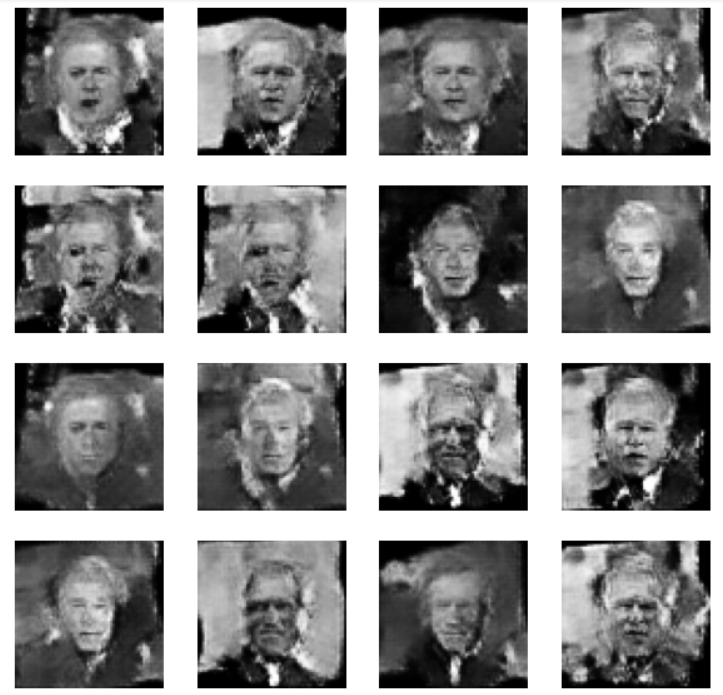
\includegraphics[width=0.7\linewidth]{images/sample.png}
    %\vspace{1em}
    \caption{Przykładowy obrazek}
    \label{fig:pdgd}
    \source{Opracowanie własne}
\end{figure}


\end{document}
